\chapter {Release 3 : Gestion des projets et utilisateurs}

\section{Introduction} 
Ce cinquième et dernier chapitre présente la troisième release de notre application, centrée sur la gestion des projets et des utilisateurs. Le sprint 5 a permis l’intégration des projets depuis GitLab et la collecte des logs CI/CD pour une analyse automatisée par le modèle d’IA. Le sprint 6 a introduit la gestion des rôles et des états des utilisateurs, renforçant le contrôle et la sécurité de la plateforme.

Nous présentons ici le backlog, les diagrammes de cas d’utilisation et de classes, les descriptions textuelles, les diagrammes de séquence ainsi que les interfaces réalisées, illustrant la mise en œuvre de ces fonctionnalités de manière claire et structurée.

\section{Sprint 5}
\subsection{Objectifs du sprint 5}
L’objectif de ce sprint est de permettre aux utilisateurs d’ajouter des projets depuis GitLab et de collecter les logs des pipelines CI/CD afin de les regrouper sous forme de batch. Ces données seront ensuite mises à disposition pour une analyse par le modèle d’IA, ce qui facilitera la détection d’anomalies et l’amélioration du suivi des pipelines.
\subsection{Backlog sprint 5}

\begin{table}[H]
\centering
\scriptsize
\setlength{\tabcolsep}{4pt} % réduit l'espace interne des cellules
\begin{tabular}{|
>{\centering\arraybackslash}m{0.9cm}|
>{\centering\arraybackslash}m{3cm}|
>{\centering\arraybackslash}m{1.1cm}|
m{5.5cm}|
>{\centering\arraybackslash}m{1.4cm}|
>{\centering\arraybackslash}m{1.6cm}|
>{\centering\arraybackslash}m{1.3cm}|}
\hline
\textbf{ID} & \textbf{Module} & \textbf{Story ID} & \textbf{User Story} & \textbf{Priorité} & \textbf{Complexité} & \textbf{Nb jours} \\
\hline
\multirow{2}{*}{5}
& \multirow{2}{3cm}{Intégration des projets CI/CD}
& 5.1 & En tant qu’utilisateur, je veux \newline ajouter des projets depuis GitLab
& Élevée & L & 20 \\
\cline{3-7}
& & 5.2 & En tant qu’utilisateur, je veux \newline consulter les logs des pipelines CI/CD
& Élevée & L & 5 \\
\hline
\end{tabular}
\captionsetup{justification=centering}
\caption{Backlog Sprint 5}
\end{table}

Le tableau 5.1 représente le Backlog de sprint 5.

\subsection{Etude conceptuelle du sprint 5}
\subsubsection{Use case du sprint 5}
La figure 5.1 représnete le diagramme de cas d'utilisation de Sprint 5

\begin{figure}[H]
    \centering
    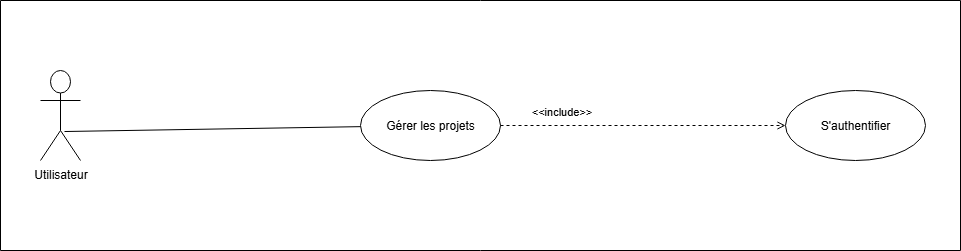
\includegraphics[width=1\linewidth]{img/usecasesprint5.png}
    \caption{use case sprint 5}
    \label{fig:enter-label}
\end{figure}


\subsubsection{Diagramme de classes sprint 5}
La figure 5.2 représente le diagramme de classes du sprint 5


\begin{figure}[H]
    \centering
    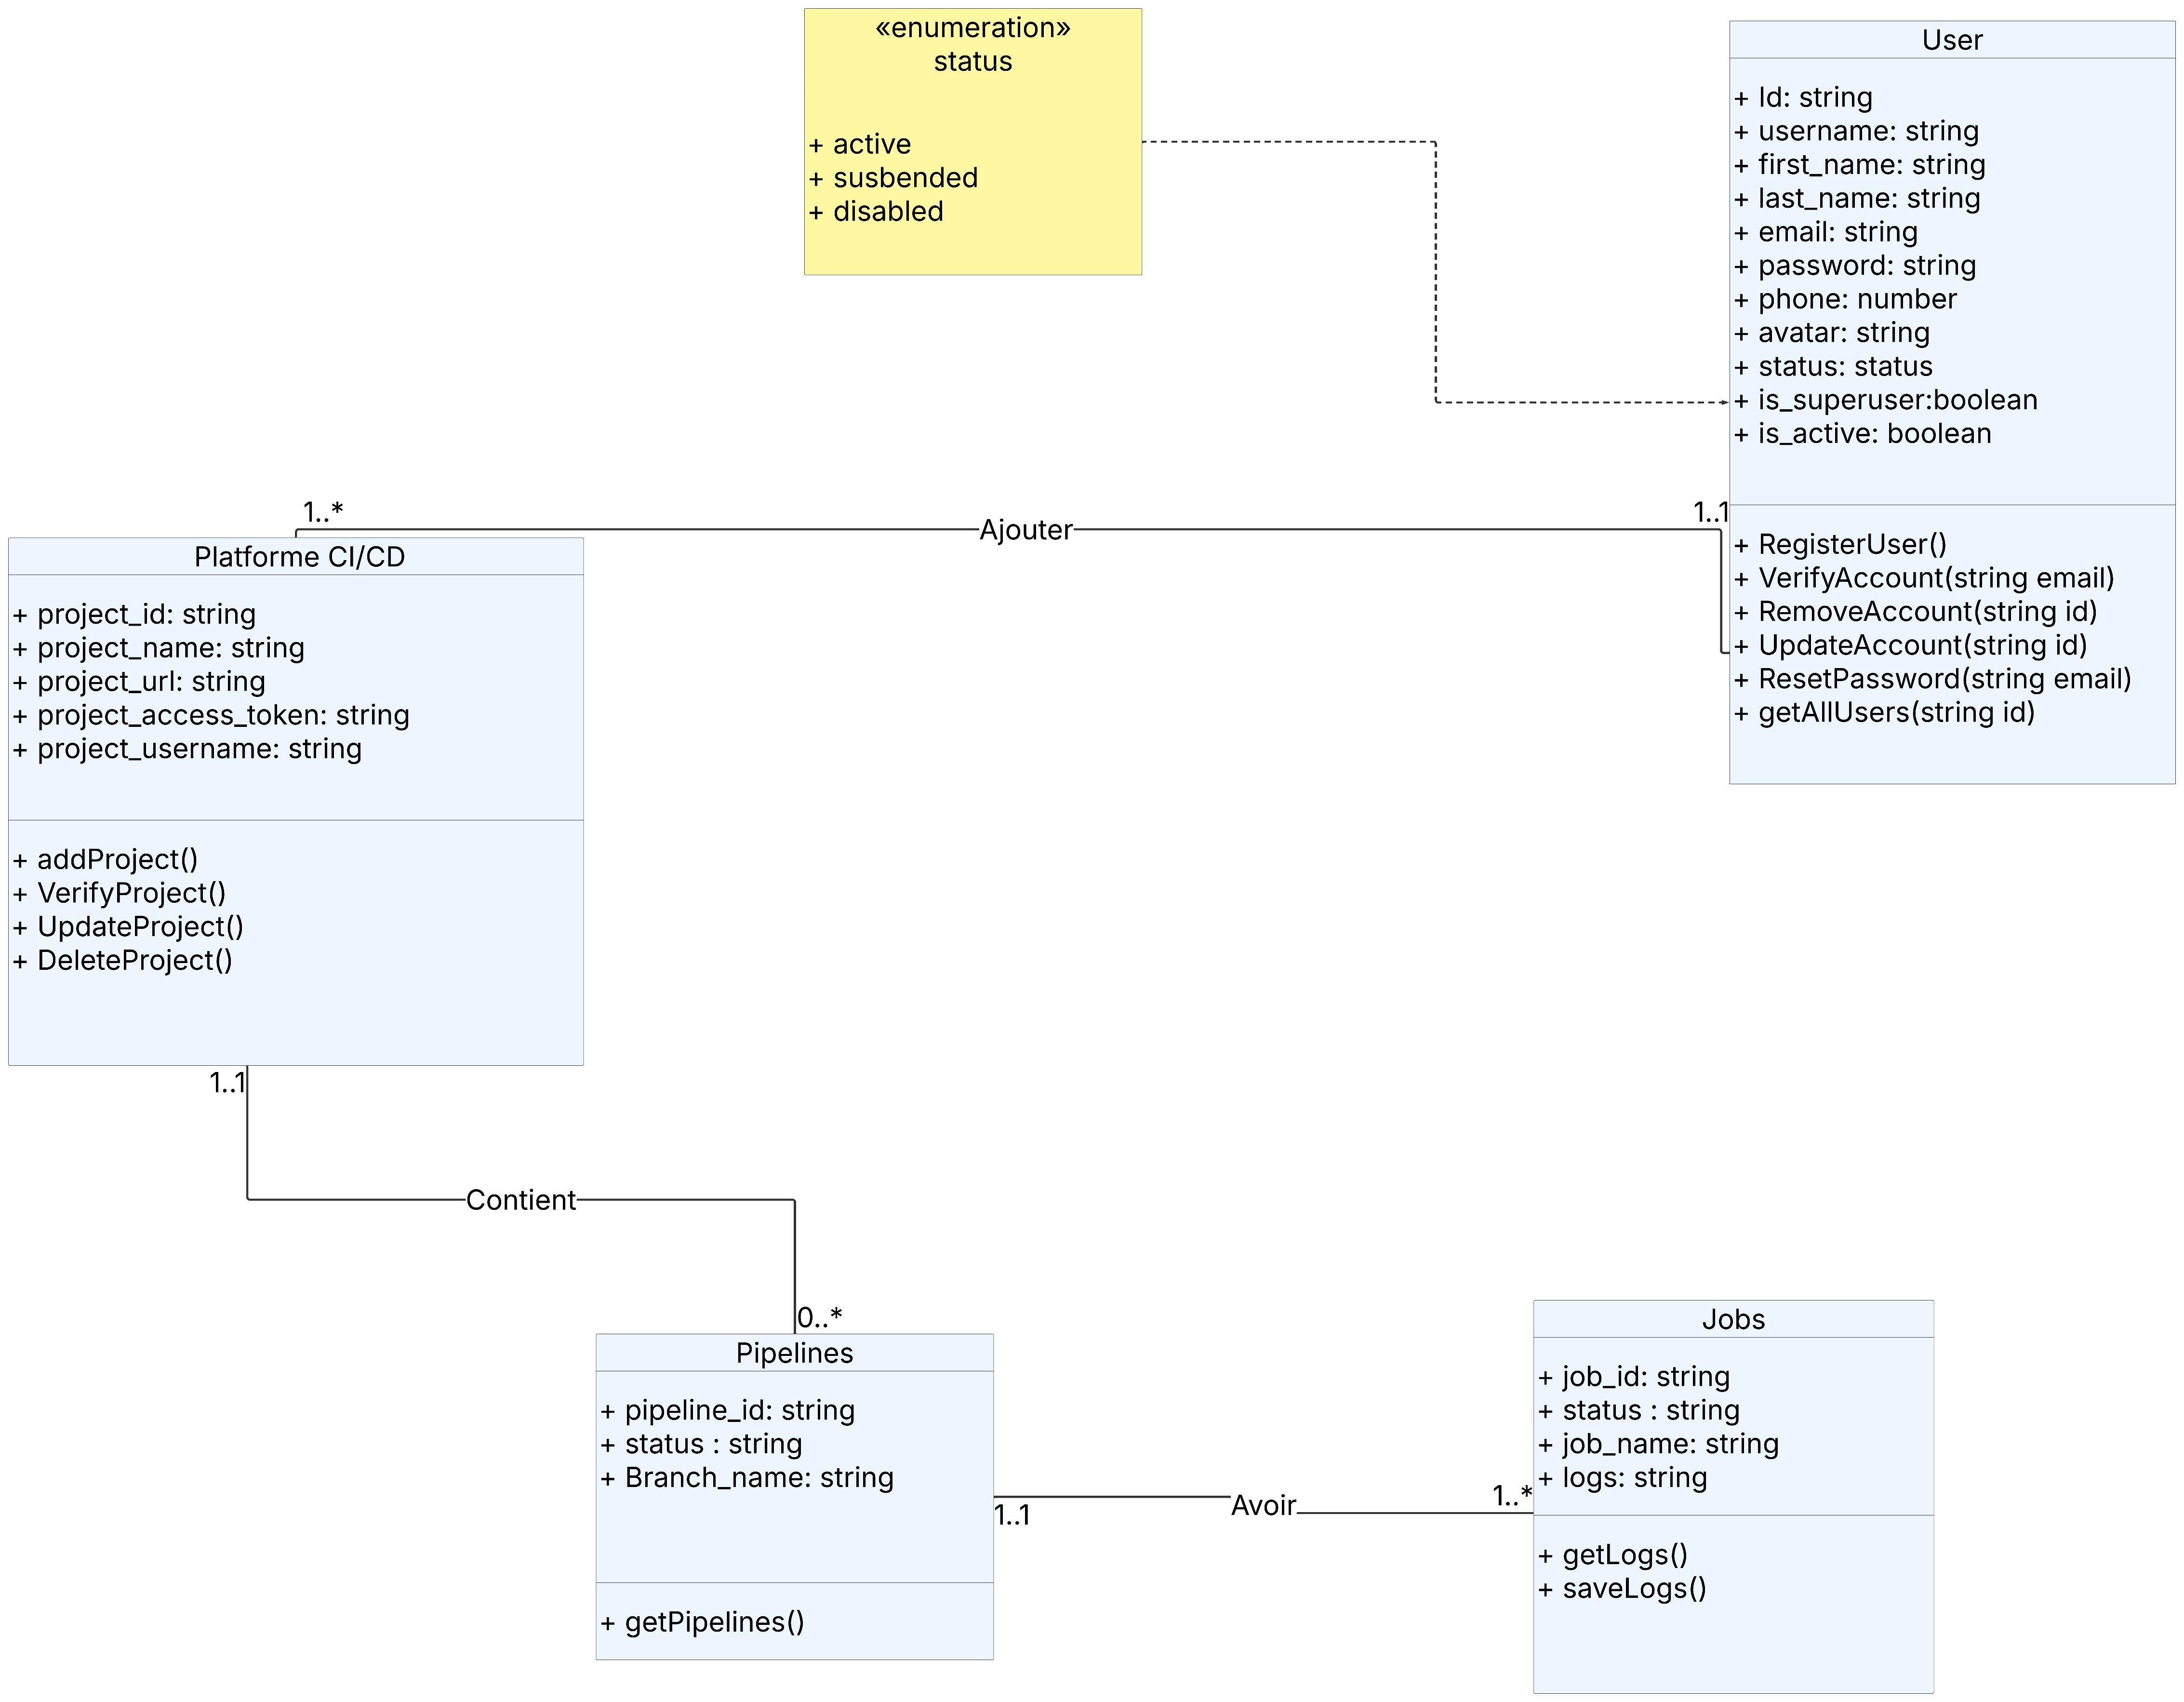
\includegraphics[width=1.15\linewidth]{img/Sprint 5 classes.jpeg}
    \caption{Sprint 5 diagramme de classes}
    \label{fig:enter-label}
\end{figure}


\subsubsection{Description textuelle de cas d'utilisation}


\begin{itemize}[label=\textbullet]
    \item \textbf{Description textuelle du cas d’utilisation Ajouter un projet}
\end{itemize} 

Le tableau 5.2 représente une description textuelle de cas d'utilisation "Ajouter un projet"

\begin{longtable}{|>{\raggedright\arraybackslash}p{4cm}|>{\raggedright\arraybackslash}p{11cm}|}
\hline
\textbf{Cas d’utilisation} & Ajouter un projet\\
\hline
\textbf{Acteur} & Utilisateur \\
\hline
\textbf{Pré-condition} & L'utilisateur doit être authentifié. \\
\hline
\textbf{Post-condition} & Le projet est ajouté et vérifié via l’API GitLab. \\
\hline
\textbf{Scénario nominal} &
1. L’utilisateur visite la page des projets. \newline
2. L’utilisateur sélectionne l’option \og Ajouter un projet \fg{}. \newline
3. L’utilisateur choisit la plateforme de gestion du code source. \newline
4. L’utilisateur saisit l’URL du projet, l’identifiant du projet, le nom d’utilisateur et le jeton d’accès. \newline
5. Le système vérifie les informations fournies en appelant l’API GitLab. \newline
6. Le projet est ajouté avec succès et visible dans la liste des projets. \\
\hline
\textbf{Scénario alternatif} &
- Projet introuvable . \newline
- Jeton d’accès expiré ou invalide. \\
\hline

\captionsetup{justification=centering}
\caption{Description textuelle du cas d’utilisation Ajouter un projet}
\label{tab:Description textuelle du cas d’utilisation Ajouter un projet}
\end{longtable}

\begin{itemize}[label=\textbullet]
    \item \textbf{Diagramme de séquence ajouter projet}
\end{itemize} 
La figure 5.3 présente le diagramme de séquence "Ajouter projet"

\begin{figure}[H]
    \centering
    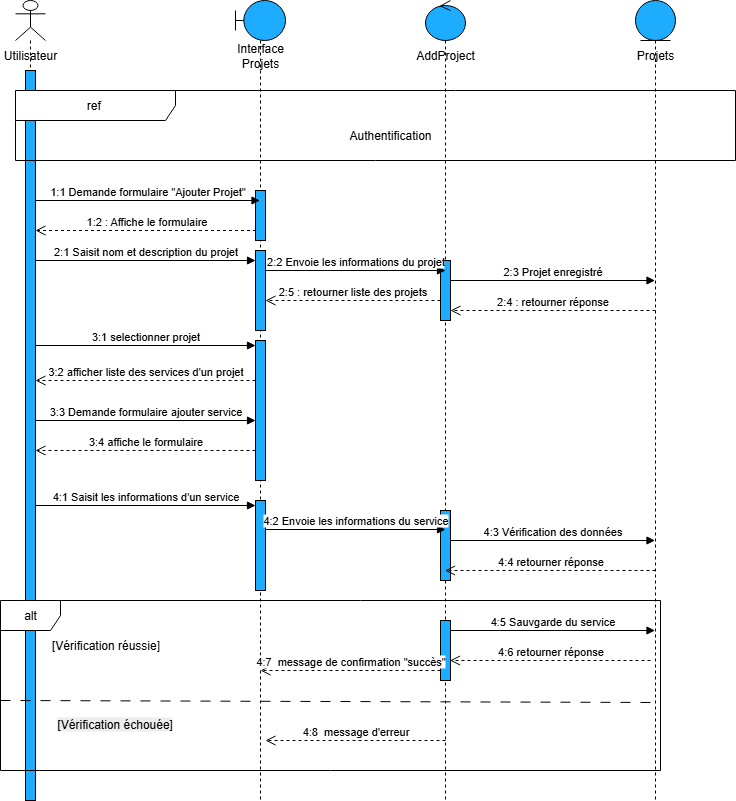
\includegraphics[width=1\linewidth]{img/addprojectseq.png}
    \caption{Sprint 5 diagramme de séquence "Ajouter Projet"}
    \label{fig:enter-label}
\end{figure}



\begin{itemize}[label=\textbullet]
    \item \textbf{Description textuelle du cas d’utilisation Consulter les logs des pipelines CI/CD}
\end{itemize} 
Le tableau 5.3 représente le cas d'utilisation consulter les logs CI/CD
\begin{longtable}{|>{\raggedright\arraybackslash}p{4cm}|>{\raggedright\arraybackslash}p{11cm}|}
\hline
\textbf{Cas d’utilisation} & Consulter les logs des pipelines CI/CD \\
\hline
\textbf{Acteur(s)} & Utilisateur
\\
\hline
\textbf{Pré-condition} & 
L’utilisateur doit être authentifié .  \newline Des batchs doivent exister pour pouvoir consulter les logs.. \\
\hline
\textbf{Post-condition} & 
Les logs CI/CD du batch sélectionné sont affichés. \\
\hline
\textbf{Scénario nominal} &
1. L’utilisateur accède à la page \og Data \fg{} contenant la liste des batchs. \newline
2. L’utilisateur sélectionne un batch spécifique. \newline
3. L’utilisateur choisit l’option \og CI/CD Logs \fg{} pour filtrer les données. \newline
4. Les logs CI/CD sont affichés dans l’interface. \\
\hline
\textbf{Scénario alternatif} &
- Aucun batch n’est disponible. \newline
- Aucun pipeline associé au batch sélectionné. \newline
- Échec de récupération des logs depuis l’API .
\\
\hline


\captionsetup{justification=centering}
\caption{Description textuelle du cas d’utilisation Consulter les logs des pipelines CI/CD}
\label{tab:Description textuelle du cas d’utilisation Consulter les logs des pipelines CI/CD}
\end{longtable}

\subsection{Réalisation du Sprint 5}
Dans cette section nous allons présenter les interfaces réalisées pour Sprint 5
\begin{itemize} [label=\textbullet]

\item \textbf {Interfaces projets}

Ces interfaces présente les différents étapes pour ajouter un projet a partir d'un SCM plateforme

\item \textbf {Interface ajouter première étape :}

La figure 5.4 représente la première étape d'ajout d'un projet l'utilisateur doit sasit d'abord un nom a un projet avec une description :
\begin{figure}[H]
    \centering
    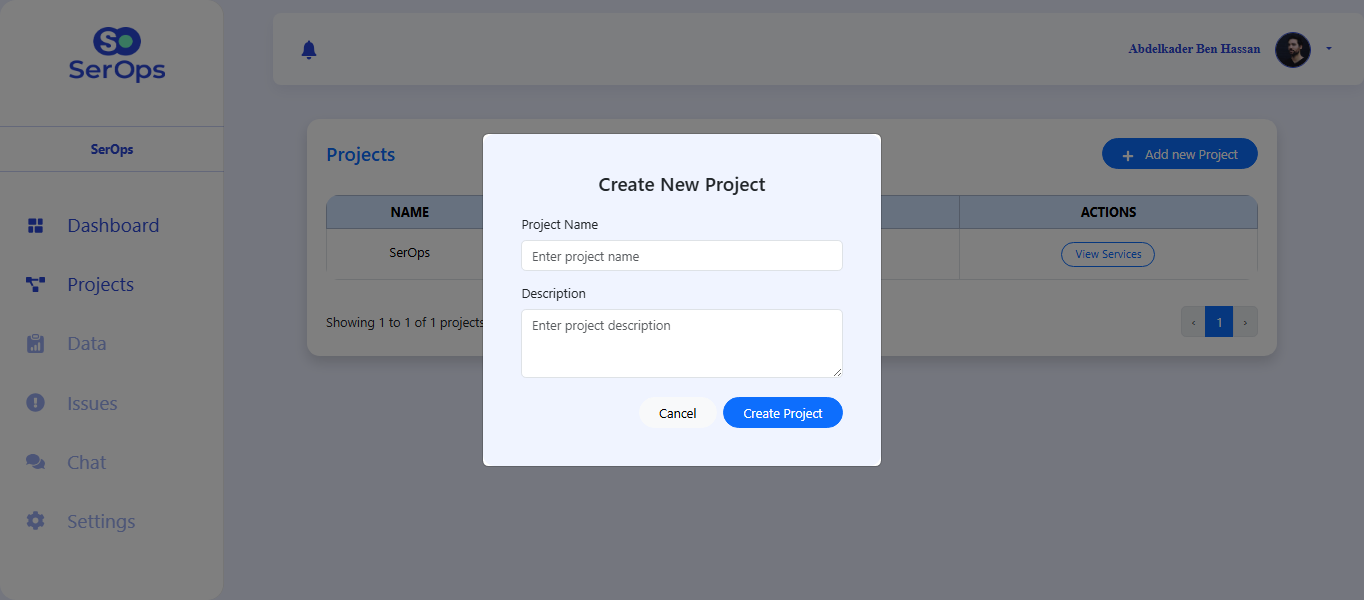
\includegraphics[width=1\linewidth]{img/addporojectstp1.png}
    \caption{Interface Ajouter projet étape 1}
    \label{fig:enter-label}
\end{figure}

\clearpage

\item \textbf {Interface ajouter deuxième étape}

La figure 5.5 représente la deuxième étape d'ajout d'un projet l'utilisateur doit selectioner un type de service et la platfrom de source code managment :
\begin{figure}[H]
    \centering
    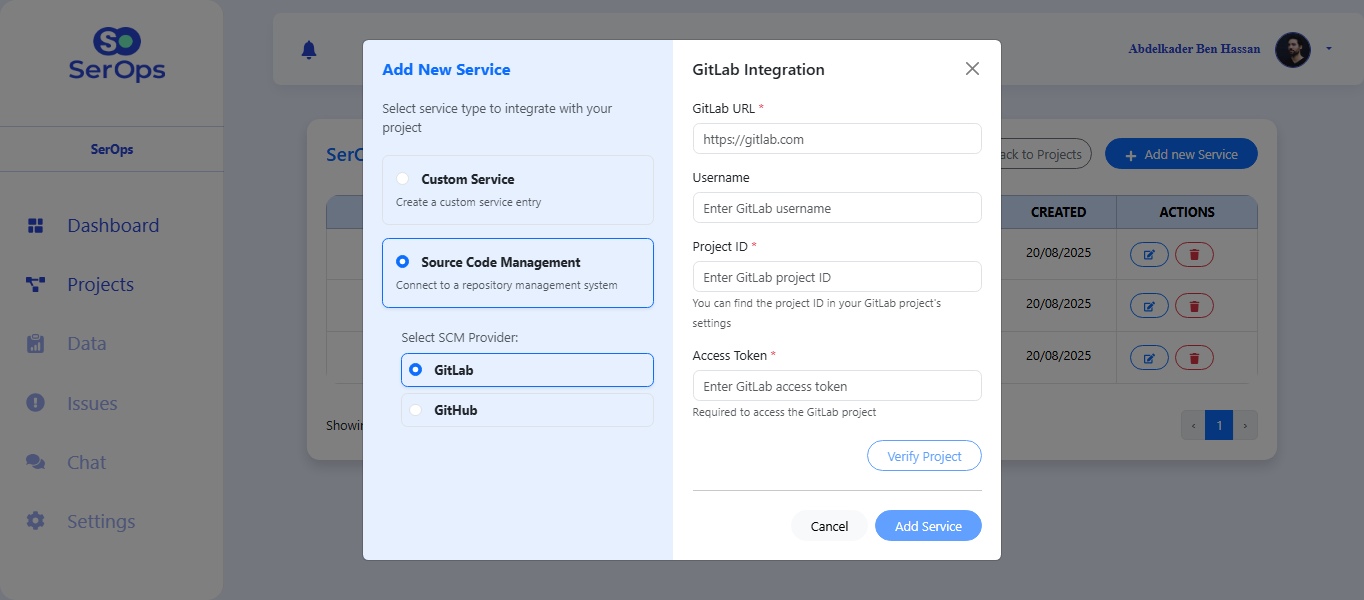
\includegraphics[width=1\linewidth]{img/addprojectstp2.png}
    \caption{Interface Ajouter projet étape 2}
    \label{fig:enter-label}
\end{figure}

\item \textbf {Interface verifier projet gitlab}

La figure 5.6 représente la vérification du projet gitlab après la saisie des données

\begin{figure}[H]
    \centering
    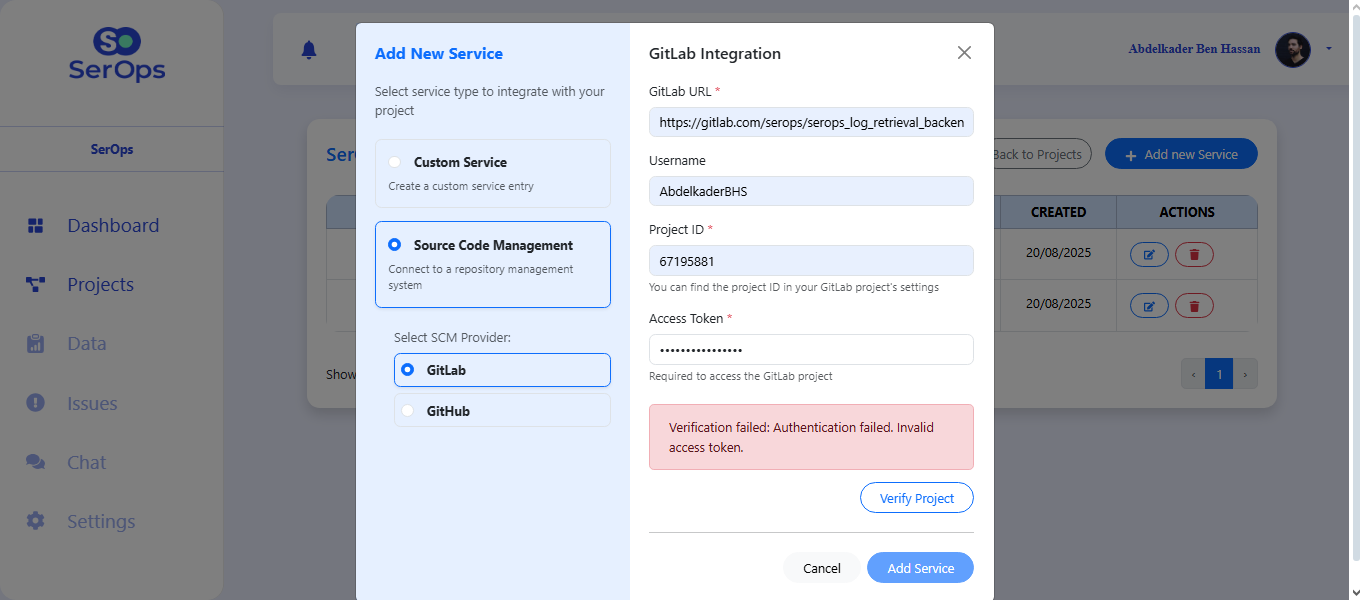
\includegraphics[width=1\linewidth]{img/verifyservice.png}
    \caption{Interface vérifier service}
    \label{fig:enter-label}
\end{figure}


\item \textbf {Interface liste des services}

La figure 5.7 représente la liste des services d'un projet :
\begin{figure}[H]
    \centering
    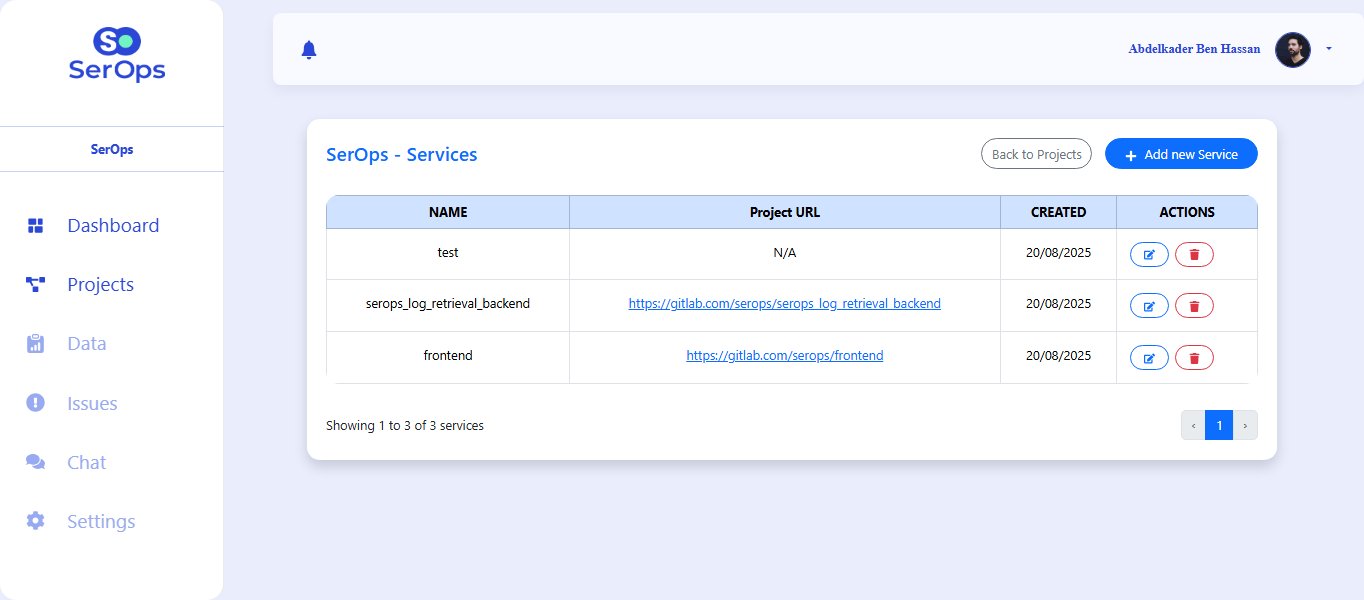
\includegraphics[width=1\linewidth]{img/listeservices.png}
    \caption{Interface liste services}
    \label{fig:enter-label}
\end{figure}
\end{itemize}



\section{Sprint 6}
\subsection{Objectifs du sprint 6}

L’objectif principal de ce sprint est de mettre en place les fonctionnalités nécessaires pour permettre aux administrateurs de gérer efficacement les utilisateurs du système. 
Plus précisément, il s’agit d’introduire la gestion des rôles (par exemple, devops, développeur, admin etc.) ainsi que la gestion des états des comptes utilisateurs 
(actif, inactif, suspendu). Ces fonctionnalités visent à renforcer le contrôle et la sécurité de la plateforme, tout en offrant une meilleure flexibilité dans 
l’administration des droits d’accès.

\subsection{Backlog Sprint 6}

\begin{table}[H]
\centering
\scriptsize
\setlength{\tabcolsep}{4pt}
\begin{tabular}{|
>{\centering\arraybackslash}m{0.9cm}|
>{\centering\arraybackslash}m{3cm}|
>{\centering\arraybackslash}m{1.1cm}|
m{5.5cm}|
>{\centering\arraybackslash}m{1.4cm}|
>{\centering\arraybackslash}m{1.6cm}|
>{\centering\arraybackslash}m{1.3cm}|}
\hline
\textbf{ID} & \textbf{Module} & \textbf{Story ID} & \textbf{User Story} & \textbf{Priorité} & \textbf{Complexité} & \textbf{Nb jours} \\
\hline
\multirow{4}{*}{6}
& \multirow{4}{3cm}{Gestion des utilisateurs}
& 6.1 & En tant qu’administrateur, je veux attribuer ou modifier les rôles des utilisateurs afin de contrôler leurs droits d’accès. 
& Élevée & M & 3 \\
\cline{3-7}
& & 6.2 & En tant qu’administrateur, je veux gérer les états des utilisateurs (actif, inactif, suspendu) pour contrôler l’accès au système. 
& Élevée & L & 4 \\
\cline{3-7}
& & 6.3 & En tant qu’administrateur, je veux modifier les informations des utilisateurs.
& Élevée & M & 2 \\
\cline{3-7}
& & 6.4 & En tant qu’administrateur, je veux supprimer des utilisateurs.
& Élevée & M & 2 \\
\hline
\end{tabular}

\captionsetup{justification=centering}
\caption{Backlog Sprint 6}
\end{table}

Le tableau 5.4 représente le backlog du sprint 6.

\subsection{Etude conceptuelle du sprint 6}
\subsubsection{Use case Sprint 6}
La figure 5.8 représente le use case du sprint 6

\begin{figure}[H]
    \centering
    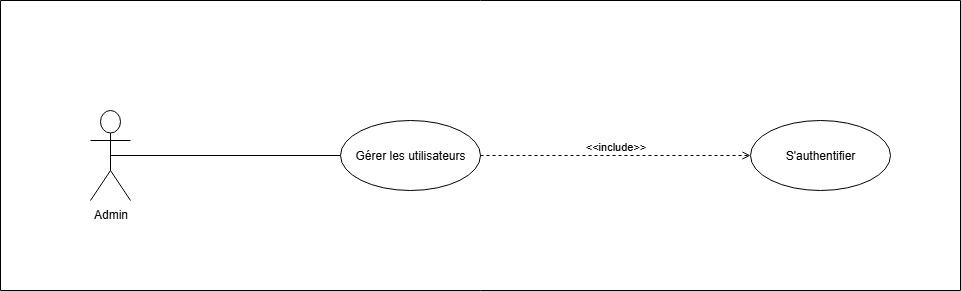
\includegraphics[width=1\linewidth]{img/sprint6usecase.jpg}
    \caption{use case sprint 6}
    \label{fig:enter-label}
\end{figure}

\subsubsection{Diagramme de classes Sprint 6}
La figure 5.8 presénte le digramme de classes du sprint 6
\begin{figure}[H]
    \centering
    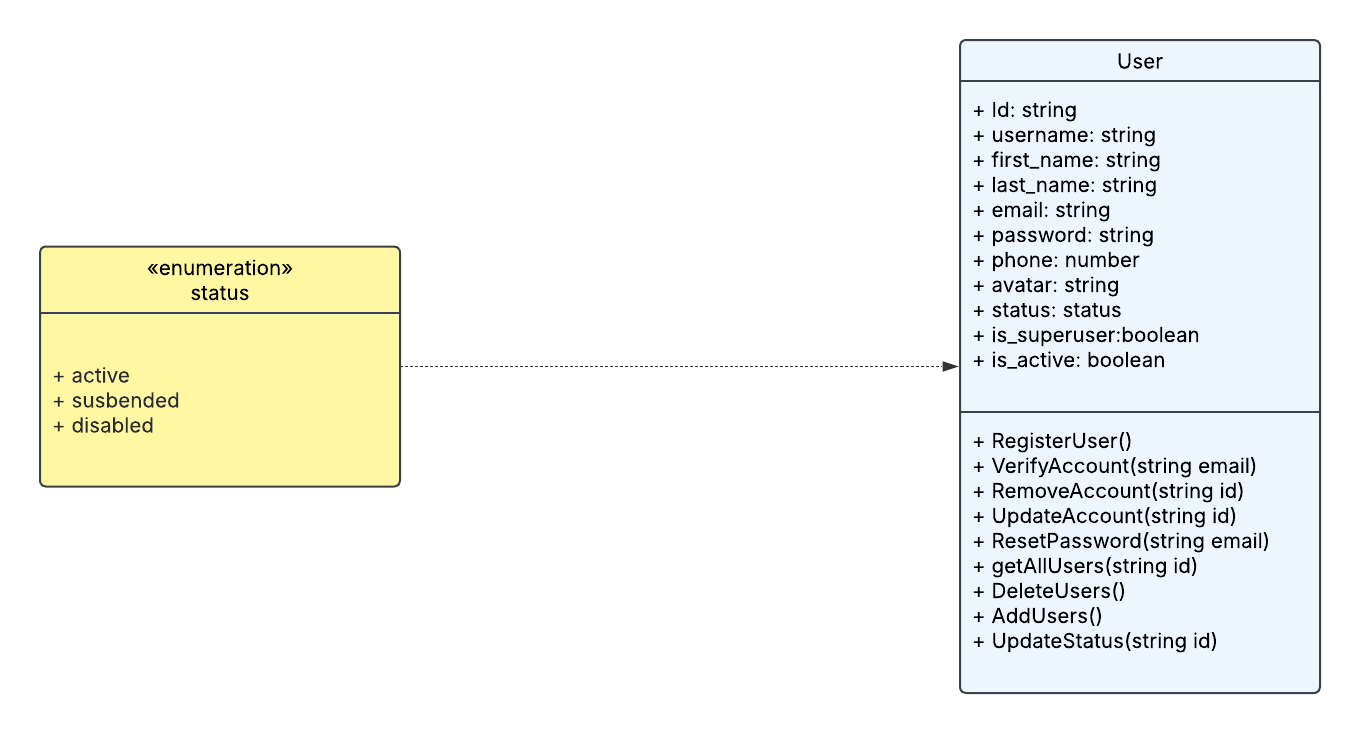
\includegraphics[width=1.15\linewidth]{img/Sprint6Classes.png}
    \caption{Diagramme de classes sprint 6}
    \label{fig:enter-label}
\end{figure}

\subsubsection{Description textuelle de cas d'utilisation du sprint 6}

\begin{itemize}[label=\textbullet]
    \item \textbf{Description textuelle Modifier les rôles des utilisateurs }
\end{itemize} 

Le tableau 5.5 représente la description textuelle de cas d'utilisation "Modifier les roles des utilisateurs"

\begin{longtable}{|>{\raggedright\arraybackslash}p{4cm}|>{\raggedright\arraybackslash}p{11cm}|}
\hline
\textbf{Cas d’utilisation} & Modifier les rôles des utilisateurs \\
\hline
\textbf{Acteur(s)} & Administrateur \\
\hline
\textbf{Pré-condition} & L’administrateur doit être authentifié. \newline Les utilisateurs doivent exister dans le système. \\
\hline
\textbf{Post-condition} & Les rôles des utilisateurs sont mis à jour, et les droits d’accès correspondants sont appliqués. \\
\hline
\textbf{Scénario nominal} &
1. L’administrateur accède à la section de gestion des utilisateurs. \newline
2. L’administrateur sélectionne un utilisateur. \newline
3. L’administrateur choisit ou modifie le rôle de l’utilisateur. \newline
4. Le système enregistre la modification et confirme la mise à jour. \\
\hline
\textbf{Scénario alternatif} &
- L’utilisateur sélectionné n’existe plus. \newline
\\
\hline

\captionsetup{justification=centering}
\caption{Description textuelle du cas d’utilisation modifier les rôles des utilisateurs}
\label{tab:DescriptionRolesUtilisateurs}
\end{longtable}

\begin{itemize}[label=\textbullet]
    \item \textbf{Description textuelle supprimer des utilisateurs }
\end{itemize}

Le tableau 5.6 représente la description textuelle du cas d'utilistion "supprimer des utilisateurs"

\begin{longtable}{|>{\raggedright\arraybackslash}p{4cm}|>{\raggedright\arraybackslash}p{11cm}|}
\hline
\textbf{Cas d’utilisation} & Supprimer des utilisateurs \\
\hline
\textbf{Acteur(s)} & Administrateur \\
\hline
\textbf{Pré-condition} & L’administrateur doit être authentifié. \newline Les utilisateurs doivent exister dans le système. \\
\hline
\textbf{Post-condition} & Les utilisateurs sélectionnés sont supprimés du système et n’ont plus accès. \\
\hline
\textbf{Scénario nominal} &
1. L’administrateur accède à la section de gestion des utilisateurs. \newline
2. L’administrateur sélectionne un ou plusieurs utilisateurs. \newline
3. L’administrateur confirme la suppression. \newline
4. Le système supprime les utilisateurs et confirme l’opération. \\
\hline
\textbf{Scénario alternatif} &
- L’utilisateur sélectionné n’existe plus. \newline
- Erreur serveur. \newline
\\
\hline

\captionsetup{justification=centering}
\caption{Description textuelle du cas d’utilisation Supprimer des utilisateurs}
\label{tab:DescriptionSupprimerUtilisateurs}
\end{longtable}

\begin{itemize}[label=\textbullet]
    \item \textbf{Diagramme de séquence supprimer les utilisateurs}
\end{itemize} 
La figure 5.10 présente le diagramme de séquence "Supprimer les utilisateurs"

\begin{figure}[H]
    \centering
    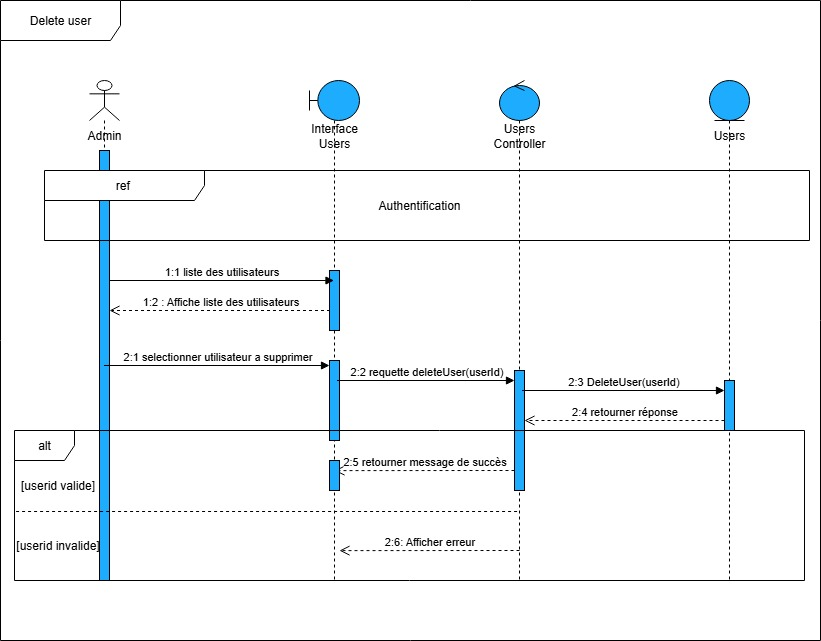
\includegraphics[width=1\linewidth]{img/deleteusersseqfinaljpg.jpeg}
    \caption{diagramme de séquence supprimer les utilisateurs}
    \label{fig:enter-label}
\end{figure}

\subsection{Réalisation du Sprint 6}
Dans cette section nous allons présenter les interfaces réalisées pour Sprint 6

\begin{itemize}[label=\textbullet]

\item  \textbf{Interface liste des utilisateurs}

La figure 5.11 représente la liste des utilisateurs

\begin{figure}[H]
    \centering
    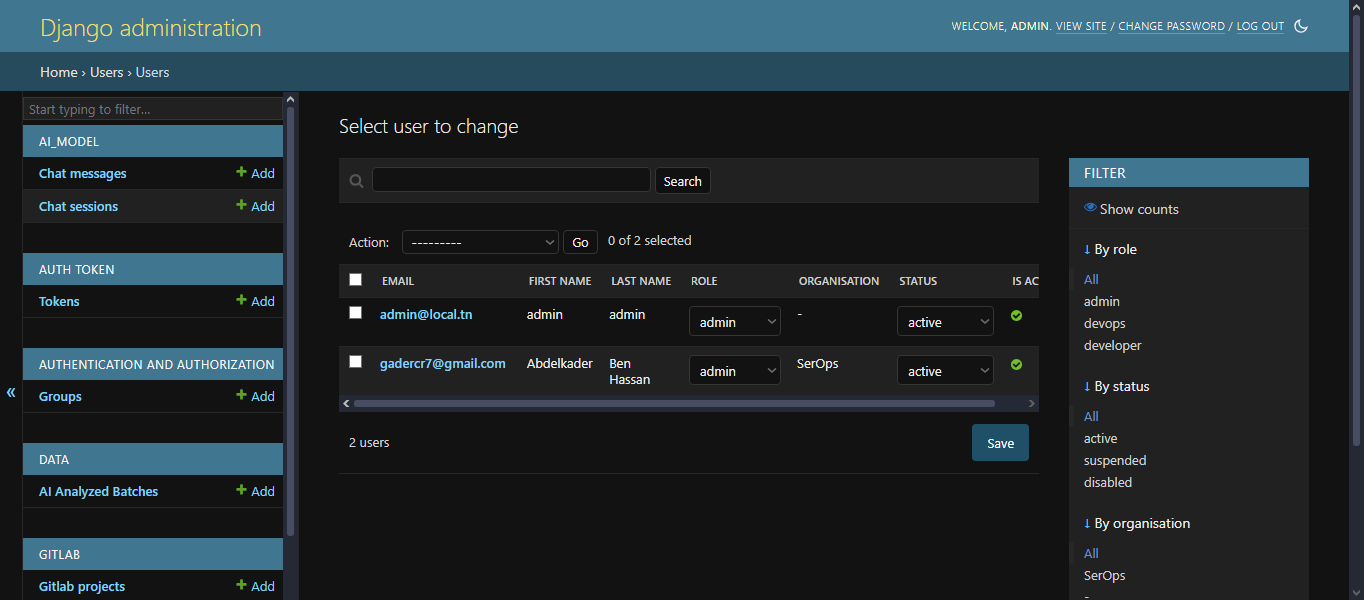
\includegraphics[width=1\linewidth]{img/Delete users.png}
    \caption{Interface liste des utilisateur}
    \label{fig:enter-label}
\end{figure}

\item  \textbf{Interface modifier utilisateur}

La figure 5.12 représente la page dans laquelle l'admin peut modifier les informations d'un utilisateur

\begin{figure}[H]
    \centering
    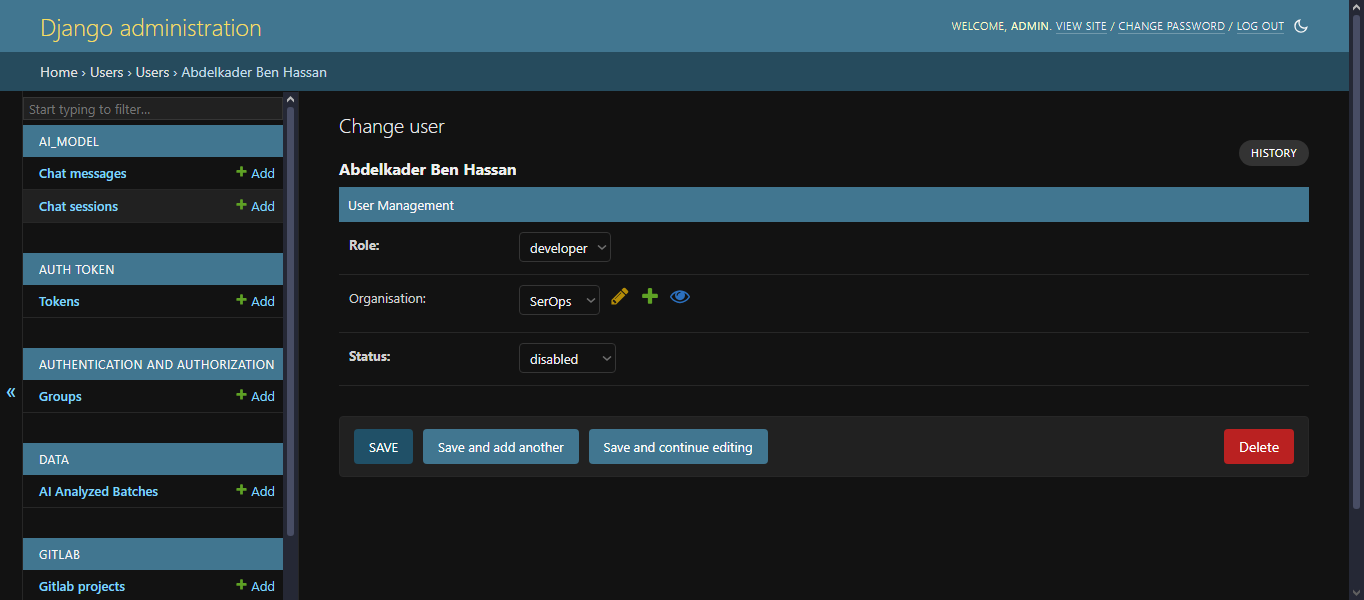
\includegraphics[width=1\linewidth]{img/editusers.png}
    \caption{Interface modifier utilisateur}
    \label{fig:enter-label}
\end{figure}


\end{itemize}

\clearpage

\section{Conclusion}
Ce dernier chapitre a présenté le troisième release, centré sur la gestion des projets et des utilisateurs. Le sprint 5 a permis l’intégration des projets depuis GitLab et la collecte des logs CI/CD, facilitant l’analyse des pipelines par le modèle d’IA. Le sprint 6 a introduit la gestion des rôles et des états des utilisateurs, renforçant le contrôle des accès et la sécurité de la plateforme.

Les diagrammes et les interfaces développées ont permis de structurer et d’implémenter les fonctionnalités de manière claire et efficace, offrant une expérience utilisateur intuitive. Ce release consolide ainsi les fonctionnalités clés du système, améliorant la supervision des projets et la gestion des utilisateurs, tout en préparant la plateforme à une utilisation fiable et sécurisée.